
% unml
\subsection{\texttt{un-ml-pipeline}: The machine learning pipeline} \label{ssec:un-ml-pipeline-the-machine-learning-pipeline}

\repo{un-ml-pipeline} is the main component of this project. It englobes a Python library, \texttt{unml}, as well as an API wrapping it. It functions as follows (see Figure \ref{fig:ml-pipeline}):
\todo[inline]{Connection to Neo4j}


\begin{figure}[!htb]
    \centering

    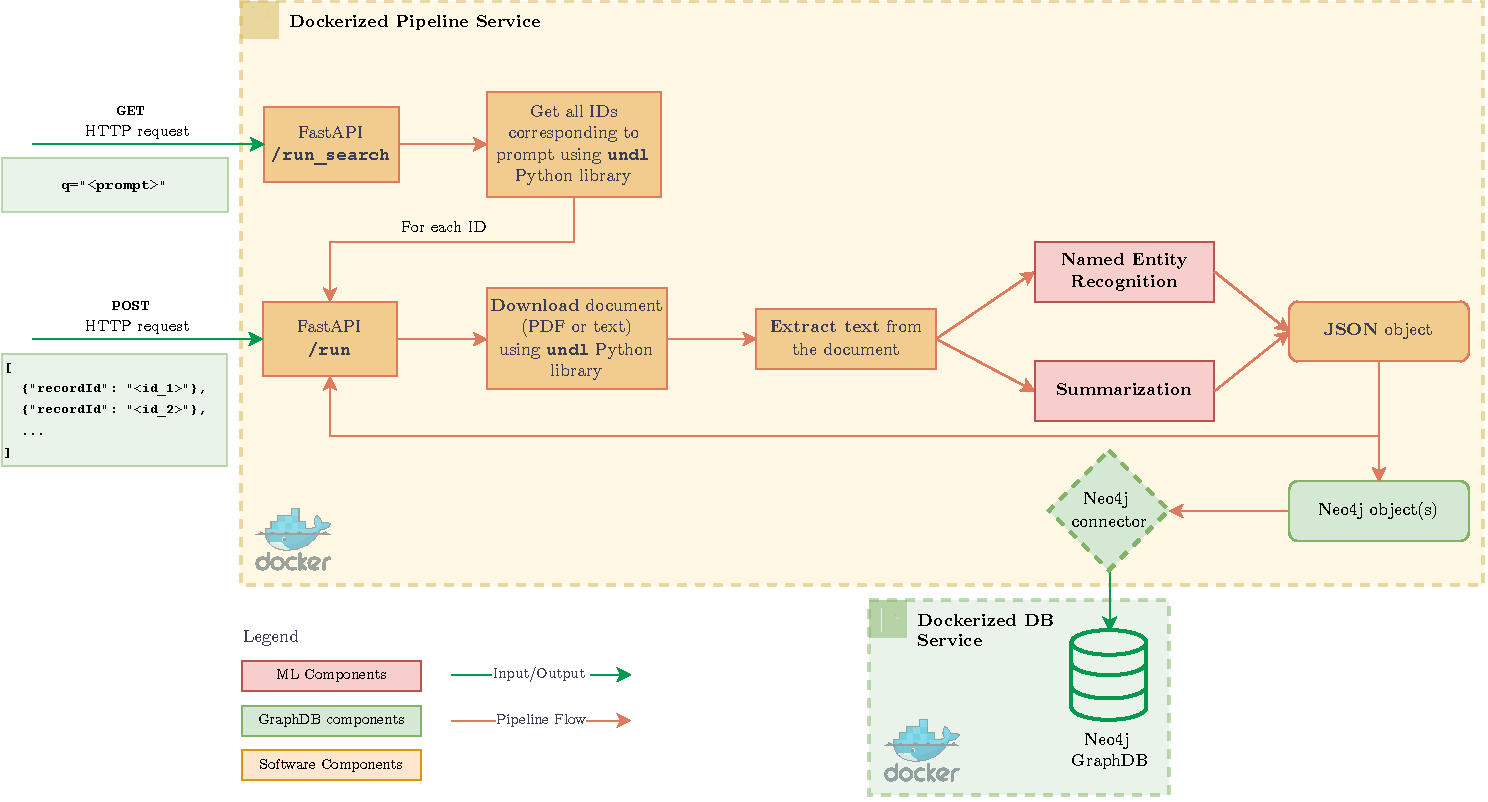
\includegraphics[width=\linewidth]{res/ml-pipeline.pdf}
    \caption{\texttt{unml} library: a dockerized machine learning pipeline for NER \& summarization}
    % change caption position to the bottom

    \label{fig:ml-pipeline}
\end{figure}

The pipeline API is a \texttt{FastAPI} app, which exposes two endpoints. The \texttt{run} endpoint gets an ID as input, and works as follows:

\begin{enumerate}
    \item A client sends an HTTP \texttt{POST} request to the pipeline API on \texttt{run} endpoint, with the payload containing a list of JSON objects with a \texttt{recordId}. (Note: this is arguably not an optimal data structure to store the IDs, but it was the easiest way to make \texttt{pydantic} happy and validate the input data structure.)

    \item Use \texttt{undl}'s client \texttt{queryBdId} method to download the corresponding document complete information and PDF document. Sometimes it doesn't exist – if it is the case, create a JSON with solely the information from the UNDL API, and jump to step $6$

    \item Extract the text from the PDF document using \texttt{PyMuPDF}\footnote{\url{https://github.com/pymupdf/PyMuPDF}} library.

    \item Then the pipeline is split into $2$ parts:
          \begin{itemize}
              \item \textbf{Named Entity Recognition}: Extract named entities from the document. All types entities are collected (the types can vary depending on the model used though), but for data quality reasons, only UN bodies and Countries are actually stored in the graph database and linked to the document. However, the other entities are still returned by the API at the end of a pipeline run, and can be used for further analysis.

              \item \textbf{Summarization}: The document is being summarized using a deep learning model, and the chosen model is a parameter of the pipeline (see Table \ref{tab:summarization-models} for more details). The summary for a document is then stored in the database to enhance the nodes.
          \end{itemize}
    \item The results of the machine learning components (e.g., the summary and the extracted named entities) are then stored into a JSON object
    \item The JSON object is converted to a Cypher (the graph database, Neo4j, query language) query and then the query is run against the Neo4j database to update the graph. Note that the Neo4j instance lives in another Docker container to better compartmentalize the stack.
\end{enumerate}


The machine learning pipeline also offers the \texttt{run\_search} endpoint, which receives a prompt as input (e.g., \texttt{"Peacekeeping"}), and works as follows:

\begin{enumerate}
    \item A client sends an HTTP \texttt{GET} request to the pipeline API on \texttt{run\_search} endpoint, with the prompt as a query parameter \texttt{q}.
    \item The pipeline API queries UNDL API against the given prompt and collects document IDs corresponding to the search results using \texttt{getAllRecordIds} method from \texttt{undl}'s. It then returns the list of IDs.
    \item For each record ID, do what querying \texttt{run} endpoint does
\end{enumerate}

\subsubsection{Models} \label{sssec:models}

When it came to choosing a model for both tasks, the main criteria were the following:
\begin{itemize}
    \item The model needs to be accurate
    \item The model needs to have fast inference due to the large number of documents the pipeline could have to deal with.
    \item The model should ideally have optimized inference for CPU, as the pipeline would preferably not be GPU-accelerated for cost reasons.
\end{itemize}

Hence, I decided to use the \texttt{transformers} library by HuggingFace, coupled with their SafeTensors\footnote{\url{https://huggingface.co/docs/safetensors/index}} technology for faster loading and \texttt{accelerate}\footnote{\url{https://huggingface.co/docs/accelerate/index}} Python library for faster inference on CPU. Some models also offered ONNX runtime binaries, but not all of them, so I didn't bother using them – this might however be a good idea for future work and to keep this pipeline cost-efficient.

For summarization, one of big challenges when choosing a model was that it should handle a very number of tokens as input. Indeed, the self-attention layer in the transformer architecture scales quadratically with the input length. Hence, transformers are often non-suited for very large inputs – and reports from the UNDL are sometimes very long and counts $100$k+ tokens. I came up with these two solutions to address this issue:

\begin{itemize}
    \item \textbf{Divide \& Conquer approach}: Recursively split and summarize the document into smaller chunks, then concatenate the summaries and pass them into the model until the length of the result summary is below fixed threshold.

    \item \textbf{Use transformers models that offer a very large input size}: Some models like LongT5 or LongFormer replace the self-attention mechanism with a custom attention mechanism that scales linearly with the input. This allows them to handle very large inputs. However, they are not as accurate as the other models, and they are also slower to train and to run inference on.
\end{itemize}

Here is a comparison of the models I used for the summarization task:

\begin{table}[!ht]
    \centering
    \small
    \begin{tabular}{p{2cm}p{2.5cm} p{2.5cm} p{2.5cm} p{2.5cm} p{2cm}}
        \toprule
                                      & \textbf{DistilBART-CNN}                                     & \textbf{DistillBART-XSUM}                                    & \textbf{DistilPegasus-CNN}                                       & \textbf{LongFormer} (\textit{default})                       & \textbf{LongT5}                                                                \\
        \midrule
        \textbf{File}                 & \github{unml/models/summarize/DistilBARTCNN.py}             & \github{unml/models/summarize/DistilBARTXSUM.py}             & \github{unml/models/summarize/DistilPegasusCNN.py}               & \github{unml/models/summarize/LED.py}                        & \github{unml/models/summarize/LongT5.py}                                       \\
        \textbf{Paper}                & \extlink{https://arxiv.org/pdf/2010.13002.pdf}{arXiv}       & \extlink{https://arxiv.org/pdf/2010.13002.pdf}{arXiv}        & \extlink{https://arxiv.org/pdf/2010.13002.pdf}{arXiv}            & \extlink{https://arxiv.org/pdf/2004.05150}{arXiv}            & \extlink{https://arxiv.org/pdf/2112.07916}{arXiv}                              \\
        \textbf{Authors}              & Shleifer et al.                                             & Shleifer et al.                                              & Shleifer et al.                                                  & Beltagy et al.                                               & Guo et al.                                                                     \\
        \textbf{Company}              & HuggingFace                                                 & HuggingFace                                                  & Google                                                           & Allen AI                                                     & Google                                                                         \\
        \textbf{Year}                 & 2020                                                        & 2020                                                         & 2020                                                             & 2020                                                         & 2022                                                                           \\
        \textbf{HuggingFace Model}    & \link{https://huggingface.co/sshleifer/distilbart-cnn-12-6} & \link{https://huggingface.co/sshleifer/distilbart-xsum-12-1} & \link{https://huggingface.co/sshleifer/distill-pegasus-cnn-16-4} & \link{https://huggingface.co/pszemraj/led-base-book-summary} & \link{https://huggingface.co/pszemraj/long-t5-tglobal-base-16384-book-summary} \\
        \textbf{Max Token Input Size} & $1'024$                                                     & $1'024$                                                      & $1'024$                                                          & $16'384$                                                     & $16'384$                                                                       \\
        \textbf{Params}               & 306M                                                        & 222M                                                         & 370M                                                             & 162M                                                         & 248M                                                                           \\
        \bottomrule
    \end{tabular}
    \caption{Models used for summarization task}
    \label{tab:summarization-models}
\end{table}



For Named Entity Recognition (NER) tasks, other models than FLERT work slightly better but are much slower due to their much larger number of parameters. In addition, spaCy has optimized inference for CPU, which is a big plus for this project. Here is a comparison of the models I used for the NER task:

\begin{table}[ht]
    \centering
    \small
    \begin{tabular}{p{4cm}p{3.2cm} p{2.5cm} p{4cm}}
        \toprule
                                   & \textbf{FLERT} (\textit{default S})                  & \textbf{RoBERTa}                                                      & \textbf{spaCy  \texttt{en\_core\_web\_trf}}         \\
        \midrule
        \textbf{File}              & \github{unml/models/ner/FLERT.py}                    & \github{unml/models/ner/RoBERTa.py}                                   & \github{unml/models/summarize/DistilPegasusCNN.py}  \\
        \textbf{Paper}             & \extlink{https://arxiv.org/abs/2011.06993}{arXiv}    & \extlink{https://arxiv.org/abs/1907.11692}{arXiv}                     & -                                                   \\
        \textbf{Authors}           & Akbik et al.                                         & Liu et al.                                                            & -                                                   \\
        \textbf{Company}           & Flair NLP                                            & Meta (fine-tune HuggingFace)                                          & spaCy                                               \\
        \textbf{Year}              & 2020                                                 & 2019                                                                  & 2023 (\texttt{v3.6.1})                              \\
        \textbf{HuggingFace Model} & \link{https://huggingface.co/flair/ner-english-fast} & \link{https://huggingface.co/Jean-Baptiste/roberta-large-ner-english} & \link{https://huggingface.co/spacy/en_core_web_trf} \\
        \textbf{Params}            & {20M(S) 560M(L)}                                     & 355M                                                                  & 355M                                                \\
        \bottomrule
    \end{tabular}
    \caption{Models used for NER task}
    \label{tab:ner-models}
\end{table}